\documentclass{beamer}

\usetheme{CambridgeUS}


\usepackage[english,greek]{babel}

\usepackage{multirow}
\usepackage{booktabs}
\usepackage{amssymb}
\usepackage{hyperref}
\setbeamertemplate{caption}[numbered]

\hypersetup{
  colorlinks=true,
  urlcolor=cyan,
  filecolor=magenta
}
\newcommand{\gr}{\selectlanguage{greek}}
\newcommand{\en}{\selectlanguage{english}}


%Information to be included in the title page:
\title[Ομάδα 30] 
{Εργασία Αναγνώρησης Προτύπων και Μηχανικής Μάθησης}


\author[Βασίλης Αϊτσίδης, Φίλιππος Ρωσσίδης]
{Βασίλης Αϊτσίδης (10330) \\ Φίλιππος Ρωσσίδης (10379) \\ Ομάδα 30}

\institute{ΑΠΘ}

\date{\today}

\begin{document}

\frame{\titlepage}


\begin{frame}
    \frametitle{Πίνακας Περιεχομένων}
    \small
    \tableofcontents[hideallsubsections]
\end{frame}

\section{ΜΕΡΟΣ Α - Εκτίμηση με Μέγιστη Πιθανοφάνεια}
\subsection{Εισαγωγή}
\begin{frame}
\frametitle{ΜΕΡΟΣ Α - Εκτίμηση με Μέγιστη Πιθανοφάνεια}

Υποθέτουμε ότι έχουμε δείγματα μιας τιμής $x$ για τα οποία θέλουμε να
αναλύσουμε κατά πόσο είναι αξιόπιστοι δείκτες του στρες για παίκτες βιντεοπαιχνιδιών.

Γνωρίζουμε ότι η πυκνότητα πιθανότητας του $x$ είναι: 
$p(x|\theta) = \frac{1}{\pi} \frac{1}{1+(x-\theta)^2}$, όπου το $\theta$ 
είναι άγνωστο. 

Γνωρίζουμε επίσης ότι από σύνολο 12 δειγμάτων: για 7 παίκτες που δεν ένιωσαν στρες (κλάση $\omega_1$)
οι δείκτες $x$ ήταν $D_1=[ 2.8, -0.4, -0.8, 2.3,-0.3,3.6,4.1]$, ενώ για τους 5 παίκτες
που ένιωσαν στρες (κλάση $\omega_2$) 
οι δείκτες $x$ ήταν $D_2=[-4.5,-3.4,-3.1,-3.0,-2.3]$. 


Για να βρούμε εάν είναι αξιόπιστος ο δείκτης $x$ θα προσπαθήσουμε να βρούμε τρόπο
να ταξινομούμε κάποιον παίκτη σε κλάσεις: στρες, όχι στρες, με τη χρήση του 
δείκτη $x$. 

Στο πρώτο μέρος θα χρησιμοποιήσουμε τη μέθοδο Μέγιστης Πιθανοφάνειας.

\end{frame}



\begin{frame}
\frametitle{Εκτίμηση με Μέγιστη Πιθανοφάνεια}

Αρχικά μπορούμε να παρατηρήσουμε (και με μια οπτικοποίηση στο σχήμα \ref{fig:1}): ότι 
οι δύο κλάσεις (για τα δείγματα που έχουμε) είναι γραμμικά διαχωρίσημες, άρα 
ήδη μπορούμε να συμπεράνουμε ότι το $x$ θα έχει σχετικά αξιόπιστα αποτελέσματα.


\begin{figure}
    \centering
        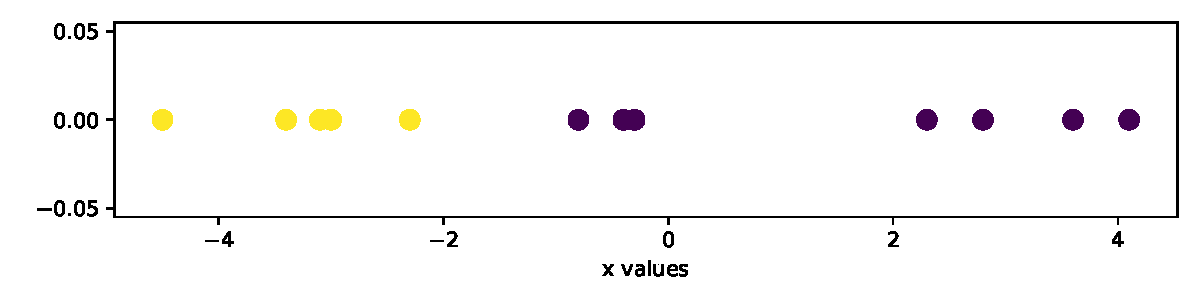
\includegraphics[width=0.7\textwidth]{../plots/Figure_1.pdf}
        \caption{Οι τιμές των δειγμάτων. Κίτρινο=στρες, μωβ=οχι στρες}
        \phantomsection
        \label{fig:1}
\end{figure}



\end{frame}

\subsection{Ερώτημα 1}
\begin{frame}
\frametitle{Εκτίμηση με Μέγιστη Πιθανοφάνεια}

Εκτιμάμε τις παραμέτρους $\hat{\theta_1}, \hat{\theta_2}$ των ΣΠΠ και για τις δύο 
κλάσεις, δηλαδή τις τιμές που μεγιστοποιούν τις (συναρτήσεις πιθανοφάνειας) $p(D_1|\theta)$ και $p(D_2|\theta)$,
αντίστοιχα.

Για διάφορες τιμές του $\theta$ υπολογίζουμε τις συναρτήσεις πιθανοφάνειας με τον τύπο:
\begin{equation}
    p(D|\theta) = p(x_1, x_2, \dots, x_N | \theta) = \prod_{n=1}^N p(x_n | \theta) 
    \label{eq:1}
\end{equation}
όπου: 
\begin{equation}
    p(x|\theta) = \frac{1}{\pi} \frac{1}{1+(x-\theta)^2}
    \label{eq:2}
\end{equation}
και $x_i \in D$.
Βρίσκουμε την τιμή $\hat{\theta}$ που μεγιστοποιεί  το $p(D|\theta)$.

Στην υλοποίηση επιλέχθηκαν 500 τιμές για το $\theta$ ομοιόμορφα στο διάστημα $[-60,60]$.


\end{frame}

\begin{frame}
\frametitle{Εκτίμηση με Μέγιστη Πιθανοφάνεια}

\begin{columns}

    \column{0.5\textwidth}
    
    Δεξιά παρατίθονται οι συναρτήσεις πιθανοφάνειας $p(D|\theta)$ για τις 
    δύο κλάσεις. Οι τιμές του $\theta$ που τις μεγιστοποιούν είναι η εκτίμηση
    του αλγορίθμου. Συγκεκριμένα για τα δεδομένα που έχουμε, οι τιμές είναι:
    $\hat{\theta_1} = 2.525, \hat{\theta_2} = -3.246$.

    Επίσης, να σημειωθεί ότι όσο περισσότερα είναι τα δείγματα, τόσο πιο 
    στενή θα είναι η καμπύλη $p(D|\theta)$.


    \column{0.5\textwidth}

    \begin{figure}
        \centering
            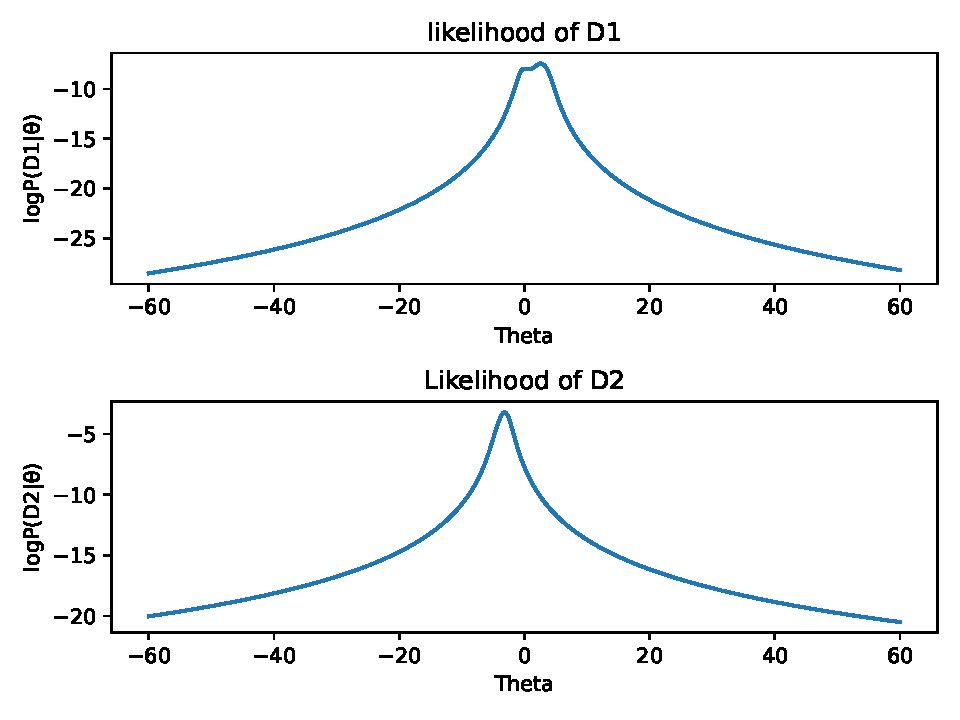
\includegraphics[width=\textwidth]{../plots/likelihoods.pdf}
            \caption{Συναρτήσεις πιθανοφάνειας για τις δύο κλάσεις.}
            \label{fig:likelihoods}
    \end{figure}


\end{columns}


    

\end{frame}

\subsection{Ερώτημα 2}

\begin{frame}
    \frametitle{Εκτίμηση με Μέγιστη Πιθανοφάνεια}
    
    Προκειμένου να ταξινομήσουμε τα $x$ σε κλάσεις χρησιμοποιούμε την συνάρτηση διάκρισης:
    \[g(x) = \log P(x | \hat{\theta}_1) - \log P(x | \hat{\theta}_2) + \log P(\omega_1) - \log P(\omega_2)\]

    Η συνάρτηση αυτή προκύπτει από τον γενικό κανόνα του \en Bayes $GBR$: \gr 
    \[\frac{p(\mathbf{x} \mid \omega_1)}{p(\mathbf{x} \mid \omega_2)} > \frac{\lambda_{12} - \lambda_{22}}{\lambda_{21} - \lambda_{11}} \frac{P(\omega_2)}{P(\omega_1)} \]
    με θεωρήσεις:

    \begin{itemize}
        \item $\lambda_{11} = \lambda_{22} = 0$, δηλαδή η ποινή σωστής ταξινόμησης είναι 0.
        \item $\lambda_{12} = \lambda_{21} = 1$, δηλαδή η ποινή λανθασμένης ταξινόμησης είναι 1.
    \end{itemize}

    αν λογαριθμίσουμε και τις δύο πλευρές.

    \begin{itemize}
        \item  $g(x) > 0 \Rightarrow P(\omega_1|x) > P(\omega_2|x)$, αρά κατατάσουμε το $x$ στην $\omega_1$.
        \item $g(x) < 0 \Rightarrow P(\omega_1|x) <  P(\omega_2|x)$ , αρά κατατάσουμε το $x$ στην $\omega_2$.
    \end{itemize}

    
\end{frame}

\begin{frame}{Εκτίμηση με Μέγιστη Πιθανοφάνεια}
\small
    Τα παραπάνω ισχύουν έχοντας υπόψη τις εξής ερμηνείες:
    \begin{itemize}
        \item $P(x|\theta):$ Είναι η συνάρτηση πυκνότητας πιθανότητας των δεδομένων $x$, δεδομένου ότι η κατανομή τους περιγράφεται από την παραμέτρο $\theta$. Εξαρτάται από την κατανομή που υποθέτουμε ότι ακολουθούν τα δεδομένα $x$. Στην περίπτωση μας αυτή της έκφρασης \ref{eq:2}. 
        \item $P(x|\omega):$ Είναι η πιθανότητα των δεδομένων $x$, δεδομένου ότι ανήκουν στην κλάση $\omega$. Μπορεί να υπολογιστεί ως:
        \[P(x|\omega) = \int P(x|\theta) P(\theta|\omega)d\theta\]
        Όταν η $\theta$ είναι σταθερή για κάθε κλάση (εκτιμάται δηλαδή ως $\hat\theta$), τότε η $P(x|\omega)$ γίνεται $P(x|\hat\theta).$
    \end{itemize}


    Εκτιμούμε τις πιθανότητες $P(\omega_1)$, $P(\omega_2)$ ως τον λόγο τον δειγμάτων που ανήκουν στην εκάστοτε κλάση ως προς τα συνολικά δείγματα.
\end{frame}


\begin{frame}{Εκτίμηση με Μέγιστη Πιθανοφάνεια}
    \begin{columns} % Begin columns
        % First column: Text
        \begin{column}{0.6\textwidth}

            Μετά την υλοποίηση του παραπάνω μοντέλου, το χρησιμοποιήσαμε για να προβλέψουμε σε ποια κλάση θα ανήκουν 
            τα 12 δείγματα μας, δεδομένου του $x$:


        
            \textbf{Παρατηρήσεις}
            \begin{itemize}
                \item Οι τιμές της \( g(x) \) καθορίζουν την κλάση.
                \item Θετικές τιμές της \( g(x) \) αντιστοιχούν στην κλάση \( \omega_1 \).
                \item Αρνητικές τιμές της \( g(x) \)αντιστοιχούν στην κλάση \( \omega_2 \).
                \item Με μία εξαίρεση την τιμή $x=-0.8$ όπου η $g(x)$ είναι αρνητική, αλλά το 
                δείγμα ανήκει στην κλάση \( \omega_1 \).
            \end{itemize}
            
        \end{column}

        % Second column: Table
        \begin{column}{0.4\textwidth}
            \centering
            \resizebox{0.85\textwidth}{!}{%
                \begin{tabular}{rrl}
                    \toprule
                    \( x \) & \( g(x) \) & Σωστή Κλάση \\
                    \midrule
                    2.8  & 1.689205  & \( \omega_1 \) \\
                    -0.4 & 0.125017  & \( \omega_1 \) \\
                    -0.8 & -0.090887 & \( \omega_1 \) \\
                    2.3  & 1.626600  & \( \omega_1 \) \\
                    -0.3 & 0.178765  & \( \omega_1 \) \\
                    3.6  & 1.492680  & \( \omega_1 \) \\
                    4.1  & 1.344624  & \( \omega_1 \) \\
                    -4.5 & -1.145734 & \( \omega_2 \) \\
                    -3.4 & -1.401339 & \( \omega_2 \) \\
                    -3.1 & -1.358416 & \( \omega_2 \) \\
                    -3.0 & -1.326927 & \( \omega_2 \) \\
                    -2.3 & -0.961337 & \( \omega_2 \) \\
                    \bottomrule
                \end{tabular}
            }
        \end{column}
    \end{columns}
\end{frame}




\begin{frame}{Εκτίμηση με Μέγιστη Πιθανοφάνεια}
    \begin{figure}
        \centering
            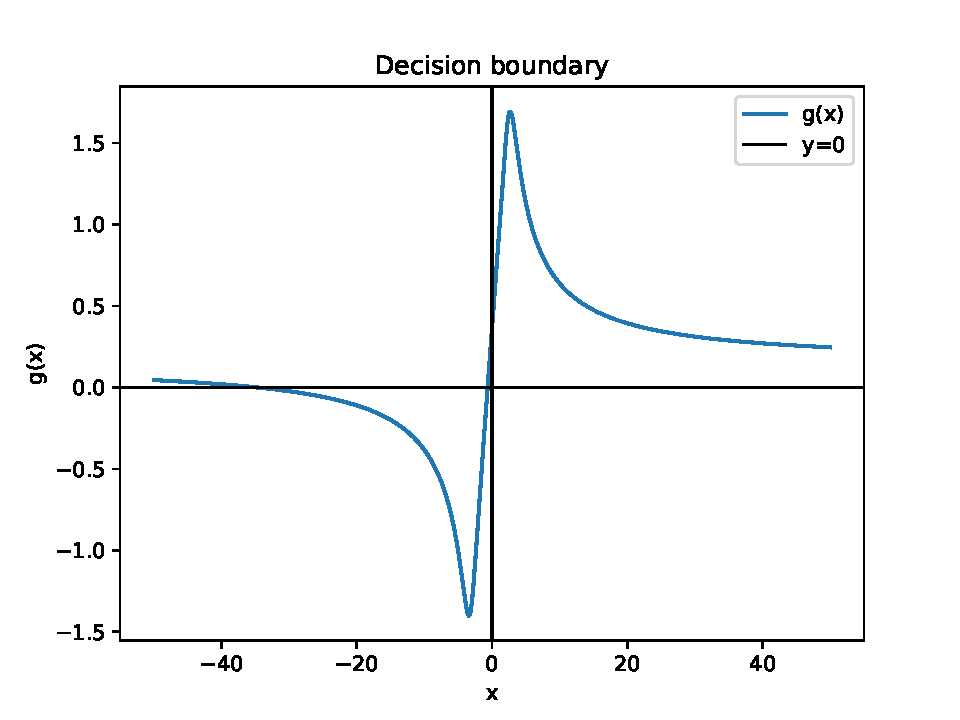
\includegraphics[width=0.6\textwidth]{../plots/DB1.pdf}
            \caption{$g(x)$ ως προς $x$. Φαίνονται οι περιοχές απόφασης του αλγορίθμου. Αν 
            η $g(x)$ είναι θετική αποφασίζουμε $\omega_1$, αλλιώς $\omega_2$. Όπως προαναφέρθηκε, 
            για $x=-0.8$ η απόφαση είναι λανθασμένη.}
            \label{fig:DB1}
    \end{figure}

    
\end{frame}



\section{ΜΕΡΟΣ Β - Μπεϋζιανή Εκτίμηση}
\subsection{Εισαγωγή}
\begin{frame}
    \frametitle{ΜΕΡΟΣ Β - Μπεϋζιανή Εκτίμηση}
    Σε αυτό το μέρος χρησιμοποιούμε το ίδιο σύνολο δεδομένων με το πρώτο μέρος, αλλά αυτή τη φορά υλοποιούμε έναν νέο ταξινομητή με τη μέθοδο εκτίμησης κατά \en Bayes. \gr H παράμετρος θ παραμένει άγνωστη, όμως τώρα γνωρίζουμε την \en prior \gr συνάρτηση πυκνότητας πιθανότητας (το οποίο αποτελεί και μια από τις βασικές διαφορές των δύο εκτιμητών): 
    \begin{equation}
        p(\theta) = \frac{1}{10\pi} \frac{1}{1+(\frac{\theta}{10})^2}
        \label{eq:3}
    \end{equation}
    
\end{frame}
\begin{frame}{Μπεϋζιανή Εκτίμηση}
    Γνωρίζοντας, λοιπόν, την \en prior \gr συνάρτηση πυκνότητας πιθανότητας αλλά και την $p(x|\theta)$ από πριν, μπορούμε σύμφωνα με τη θεωρία να εκτιμήσουμε τα εξής: 
    \begin{itemize}
        \item Υπολογισμός συνάρτησης πιθανοφάνειας $p(D|\theta)$ σύμφωνα πάλι με τον τύπο \ref{eq:1}.
        \item Υπολογισμός \en a posteriori \gr πιθανότητας σύμφωνα με τον τύπο \begin{equation}
            p(\theta|D) = \frac{p(D|\theta)p(\theta)}{\int p(D|\theta)p(\theta)d\theta}
        \end{equation}
        όπου τα $p(\theta)$ υπολογίζονται από τον τύπο \ref{eq:3}.
    \end{itemize}
\end{frame}

\subsection{Ερώτημα 1}
\begin{frame}{Μπεϋζιανή Εκτίμηση}
    \begin{columns}

    \column{0.5\textwidth}
    
    Δεξιά παρατίθενται οι καμπύλες των εκ των υστέρων πιθανοτήτων $p(\theta|D_1)$ και $p(\theta|D_2)$ για διάφορες τιμές του $\theta$. Όπως και πριν, επιλέχθηκαν 500 τιμές ομοιόμορφα στο διάστημα $[-60,60]$. 

    \column{0.5\textwidth}

    \begin{figure}
        \centering
            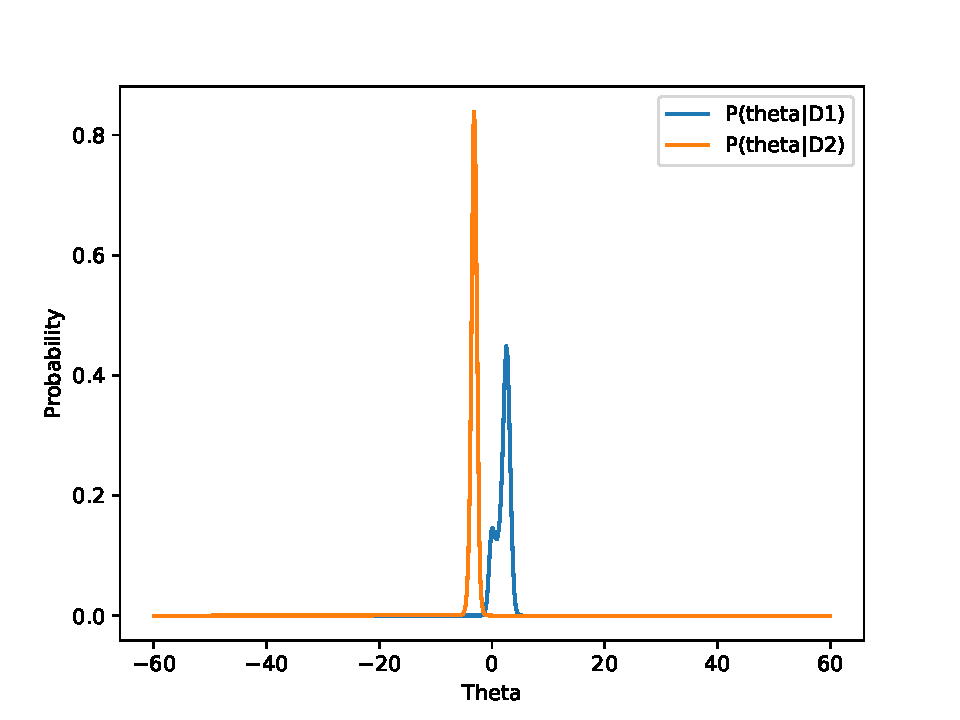
\includegraphics[width=\textwidth]{../plots/posterior.pdf}
            \caption{Απεικόνιση των \textit{εκ των υστέρων} πυκνοτήτων πιθανοτήτων για τα δύο σύνολα}
            \label{fig:posterior}
    \end{figure}


\end{columns}
\end{frame}

\begin{frame}{Μπεϋζιανή Εκτίμηση}
 \resizebox{0.85\textwidth}{!}{%
    % Top section: graphs
    \begin{columns}[T]
           \begin{columns}[T]

    \begin{column}{0.48\textwidth}
        \begin{figure}
            \centering
            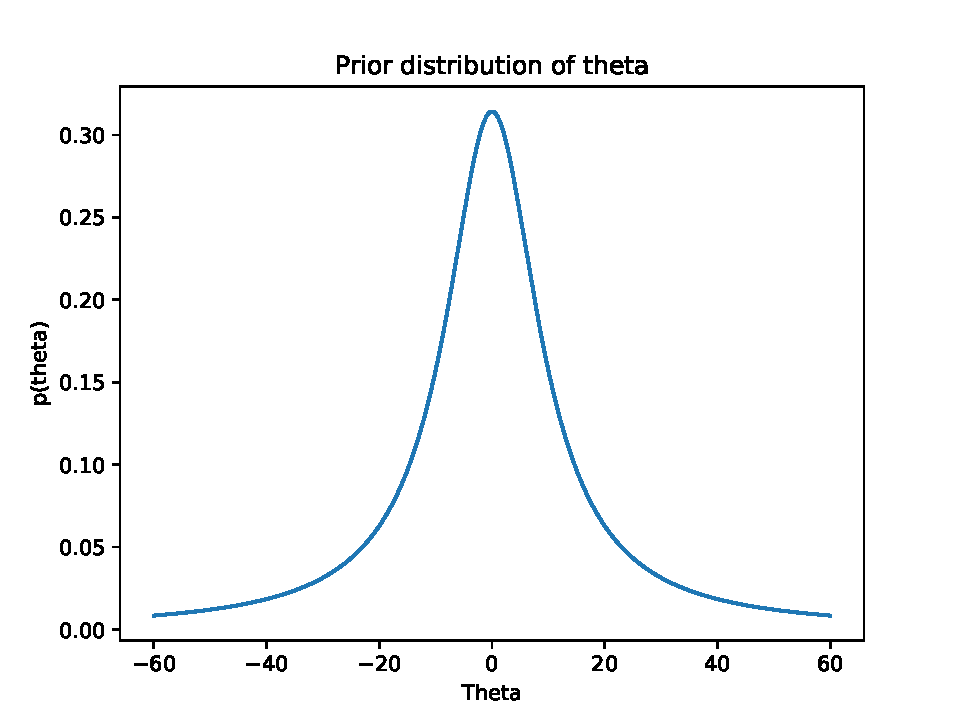
\includegraphics[width=\textwidth]{../plots/prior.pdf}
            \caption{Γράφημα της $p(\theta)$}
            \label{fig:prior}
        \end{figure}
    \end{column}

    \begin{column}{0.48\textwidth}
        \begin{figure}
            \centering
            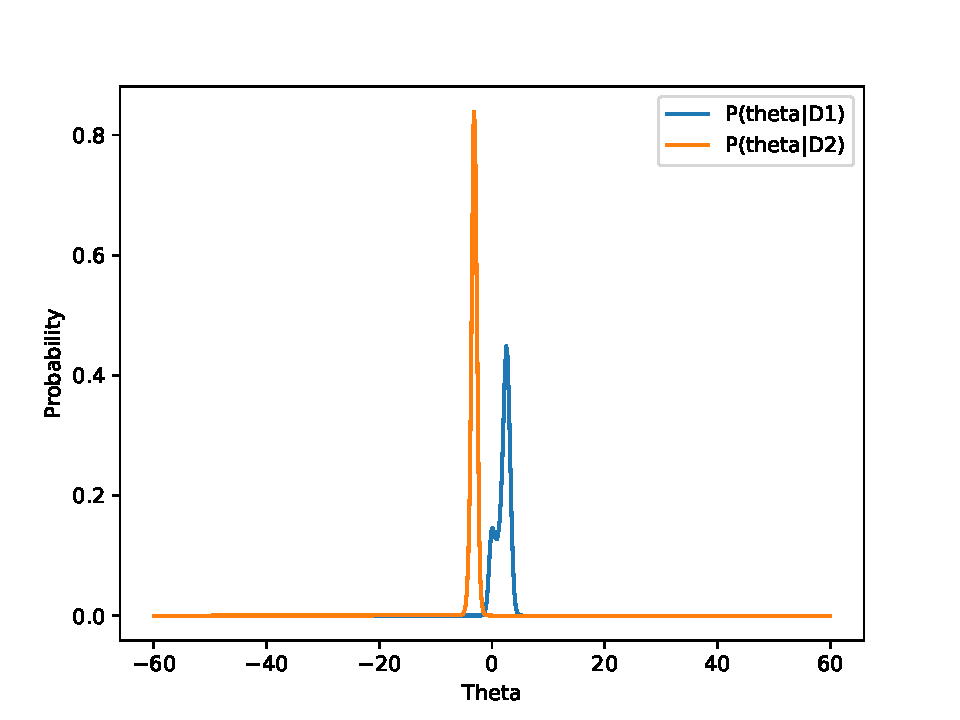
\includegraphics[width=\textwidth]{../plots/posterior.pdf}
            \caption{\en Posterior \gr κατανομές}
            \label{fig:posterior comparison}
        \end{figure}
    \end{column}
        
    \end{columns}
    \end{columns}%
    }

    % Bottom section: text
    \vfill
    \begin{columns}[T]
        \begin{column}{\textwidth}
        Συμπεράσματα: 
        \begin{itemize}
            \item Οι $p(\theta|D_1),p(\theta|D_2)$ είναι πιο συγκεντρωμένες γύρω από τις πιθανές τιμές θ που εξηγούν τα δεδομένα.
            \item Η $p(\theta)$ είναι πιο διάχυτη καθώς δεν έχει πληροφόρηση από τα δεδομένα.
        \end{itemize}
    \end{column}
    \end{columns}
\end{frame}

\subsection{Ερώτημα 2}
\begin{frame}{Μπεϋζιανή Εκτίμηση}
    Τώρα είμαστε σε θέση να υλοποιήσουμε την ταξινόμηση χρησιμοποιόντας τη συνάρτηση διάκρησης:
    \begin{equation}
        h(x) = \log P(x|D_1) - \log P(x|D_2) + \log P(\omega_1) -log P(\omega_2)
    \end{equation}
    
    Για κάθε δείγμα $x$ το οποίο θέλουμε να ταξινομήσουμε: 
    \begin{itemize}
        \item Υπολογίζουμε την $p(x|D)$ ως: \begin{equation}
        p(x|D) = \int p(x|\theta) p(\theta|D) d\theta 
    \end{equation}
    \item Υπολογίζουμε την συνάρτηση διάκρησης $h(x)$ για το $x$.
    \end{itemize}
    
\end{frame}



\begin{frame}{Μπεϋζιανή Εκτίμηση}
    Όπως και στη μέθοδο Μέγιστης Πιθανοφάνειας, έτσι κι εδώ, δίνουμε κάποιες απαραίτητες ερμηνείες:
    \begin{itemize}
        \item $P(x|\omega):$ Αυτή είναι η πιθανότητα να παρατηρηθεί το $x$, δεδομένου ότι ανήκει στην κλάση $\omega$. Αντιπροσωπεύει την πραγματική (θεωρητική) κατανομή του $x$ υπό την υπόθεση ότι το $x$ παράγεται από την κλάση $\omega$. Χρησιμοποιείται ως συνάρτηση πιθανοφάνειας στο πλαίσιο της Μπεϋζιανής Εκτίμησης.
        \item $P(x|D):$ Αυτή είναι η πιθανότητα να παρατηρηθεί το $x$, δεδομένου ότι παρατηρήθηκε το σύνολο δεδομένων $D$, το οποίο αποτελείται από δείγματα που ανήκουν στην $\omega$. Επειδή το $D$ είναι πεπερασμένο, το $P(x|D)$ αποτελεί προσέγγιση του $P(x|\omega)$. Η ακρίβεια αυτής της προσέγγισης εξαρτάται από το πόσο καλά το $D$ αναπαριστά την πραγματική κατανομή του $x$ για την $\omega$.

    \end{itemize}
\end{frame} 


\begin{frame}{Μπεϋζιανή Εκτίμηση}

    O γενικός κανόνας του \en Bayes $GBR$ \gr με τις ίδιες θεωρήσεις όπως και στο πρώτο ερώτημα, μπορεί να γραφτεί:

    \begin{equation}
        \log p(x|\omega_1) - \log p(x|\omega_2) + \log P(\omega_1) - \log P(\omega_2) > 0
    \end{equation}

    Όμως εφόσον δεν γνωρίζουμε την $p(x|\omega)$, η $p(x|D)$ είναι μια καλή εκτίμηση της. Έτσι η παραπάνω γράφεται:

    \begin{equation}
        \log p(x|D_1) - \log p(x|D_2) + \log P(\omega_1) - \log P(\omega_2) >0 \Leftrightarrow 
    \end{equation}
    \[ h(x) > 0\]

    Συγκεκριμένα, ισχύει:

    \begin{itemize}
        \item  $h(x) > 0 \Rightarrow P(\omega_1|x) > P(\omega_2|x)$, αρά κατατάσουμε το $x$ στην $\omega_1$.
        \item $h(x) < 0 \Rightarrow P(\omega_1|x) <  P(\omega_2|x)$ , αρά κατατάσουμε το $x$ στην $\omega_2$.
    \end{itemize}

    
    
\end{frame}

\begin{frame}
  \frametitle{Μπεϋζιανή Εκτίμηση}

  \begin{columns}[T]
    % Left column: text
    \begin{column}{0.5\textwidth}
        Μετά την υλοποίηση του παραπάνω μοντέλου, το χρησιμοποιήσαμε για να προβλέψουμε σε ποια κλάση θα ανήκουν 
        τα 12 δείγματα μας, δεδομένου του $x$:
        
      \textbf{Παρατηρήσεις.} \\
      \begin{itemize}
          \item Οι τιμές της $h(x)$ είναι θετικές για τα δείγματα που ανήκουν στην κλάση $\omega_1$ και αρνητικές σε αυτά που ανήκουν στην $\omega_2$. 
          \item Δεν υπάρχουν εξεραίσεις.
      \end{itemize}
    \end{column}

    % Right column: table
    \begin{column}{0.5\textwidth}
      \begin{tabular}{rrl}
        \toprule
        $x$ & $h(x)$ & Κλάση \\
        \midrule
        2.8 & 1.481023 & \(\omega_1\) \\
        -0.4 & 0.462545 & \(\omega_1\) \\
        -0.8 & 0.228873 & \(\omega_1\) \\
        2.3 & 1.422087 & \(\omega_1\) \\
        -0.3 & 0.514863 & \(\omega_1\) \\
        3.6 & 1.419364 & \(\omega_1\) \\
        4.1 & 1.312459 & \(\omega_1\) \\
        -4.5 & -1.038287 & \(\omega_2\) \\
        -3.4 & -1.162248 & \(\omega_2\) \\
        -3.1 & -1.114946 & \(\omega_2\) \\
        -3.0 & -1.088929 & \(\omega_2\) \\
        -2.3 & -0.775261 & \(\omega_2\) \\
        \bottomrule
      \end{tabular}
    \end{column}
  \end{columns}
\end{frame}



\iffalse
\begin{frame}{Μπεϋζιανή Εκτίμηση}
    \begin{figure}
        \centering
            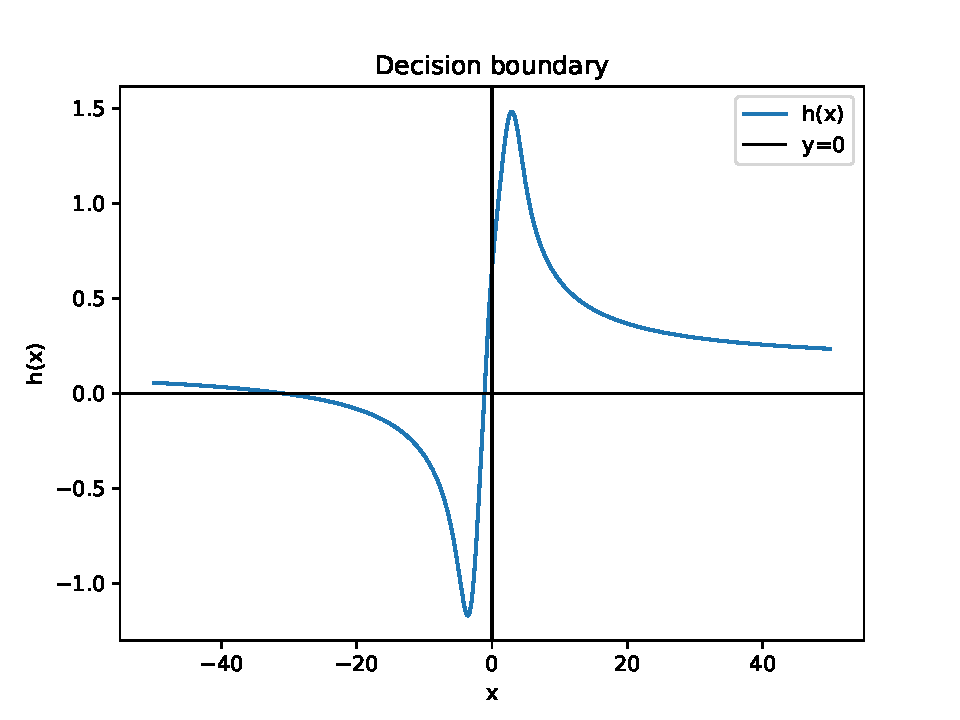
\includegraphics[width=0.6\textwidth]{../plots/DB2.pdf}
            \caption{$h(x)$ ως προς $x$. Φαίνονται οι περιοχές απόφασης του αλγορίθμου. Αν 
            η $h(x)$ είναι θετική αποφασίζουμε $\omega_1$, αλλιώς $\omega_2$.}
            \label{fig:DB2}
    \end{figure}
\fi
    
\end{frame}

\subsection{Συγκρίσεις αποτελεσμάτων Α-Β}
\begin{frame}{Σύγκριση Μέγιστης Πιθανοφάνειας και Μπεϋζιανής Εκτίμησης}
    \resizebox{0.85\textwidth}{!}{%
    % Top section: graphs
    \begin{columns}[T]
           \begin{columns}[T]

    \begin{column}{0.48\textwidth}

    \begin{figure}
        \centering
            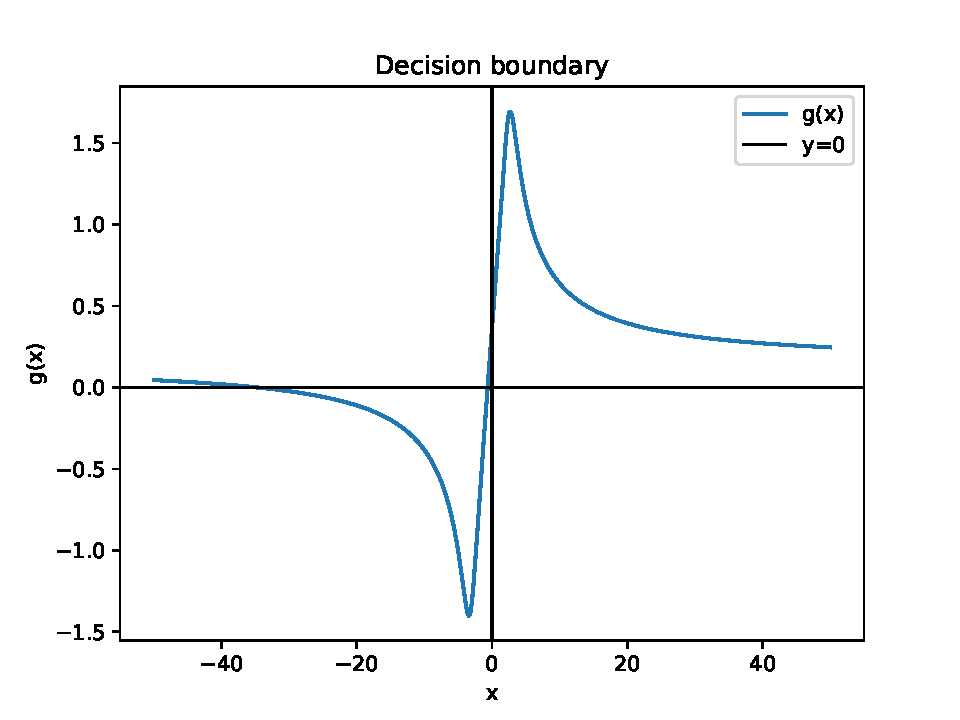
\includegraphics[width=\textwidth]{../plots/DB1.pdf}
            \caption{$g(x)$ ως προς $x$.}
            \label{fig:DB1}
    \end{figure}
        
    \end{column}

    \begin{column}{0.48\textwidth}

    \begin{figure}
        \centering
            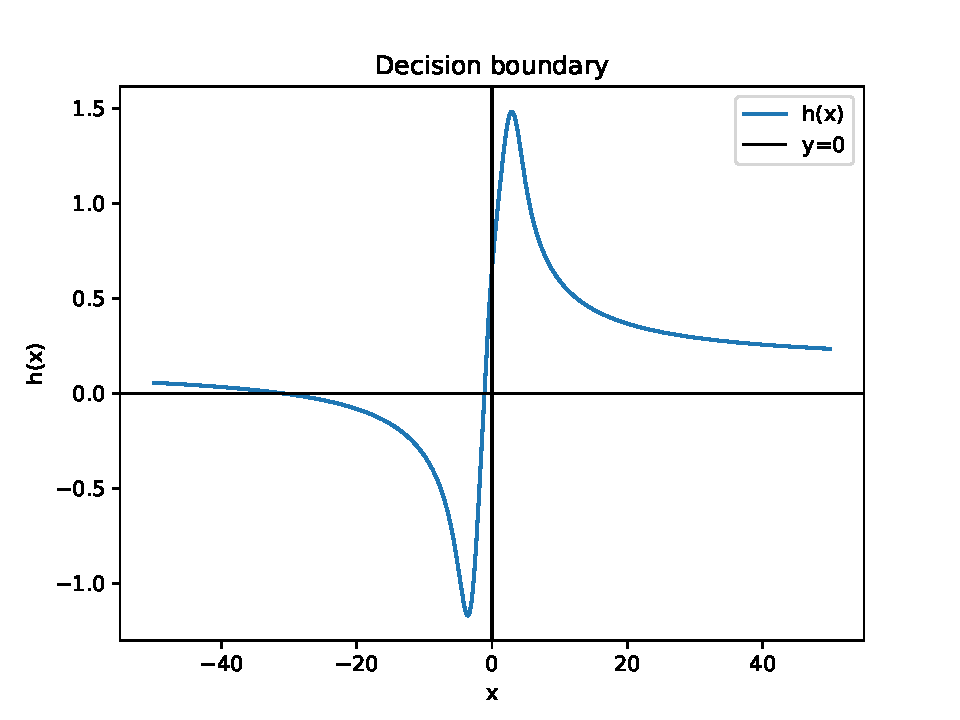
\includegraphics[width=\textwidth]{../plots/DB2.pdf}
            \tiny
            \caption{\tiny $h(x)$ ως προς $x$. Φαίνονται οι περιοχές απόφασης του αλγορίθμου. Αν 
            η $h(x)$ είναι θετική αποφασίζουμε $\omega_1$, αλλιώς $\omega_2$.}
            \label{fig:DB2}
    \end{figure}
        
    \end{column}
        
    \end{columns}
    \end{columns}%
    }

    % Bottom section: text
    \vfill
    \begin{columns}[T]
        \begin{column}{\textwidth}
            \scriptsize
            Οι περιοχές αποφάσεων της μεθόδου μέγιστης πιθανοφάνειας και μπεϋζιανής εκτίμησης είναι σχεδόν ίδιες. Όμως 
            παρατηρούμε μια διαφορά στην περιοχή κοντά του 0. Συγκεκριμένα η μπεϋζιανή εκτίμηση ταξινομεί στην κλάση 
            $\omega_1$ κάποιες πιο αρνητικές τιμές, και έτσι 'πιάνει' και το $x=-0.8$, ενώ η μέγιστης πιθανοφάνειας το 
            ταξινομεί λανθασμένα στην $\omega_2$.
        \end{column}
    \end{columns}

\end{frame}


\begin{frame}{Σύγκριση Μέγιστης Πιθανοφάνειας και Μπεϋζιανής Εκτίμησης}
\small

Ο αλγόριθμος της μπεϋζιανής εκτίμησης είναι σημαντικά πιο περίπλοκος, και ενώ στο συγκεκριμένο παράδειγμα δεν υπήρξε τέτοιο 
ζήτημα, σε παραδείγματα με περισσότερες διαστάσεις και περισσότερα δείγματα η διαφορά θα ήταν ορατή. 

Όμως η γνώση της \en prior \gr συνάρτησης πυκνότητας πιθανότητας $p(\theta)$ δίνει μεγαλύτερη ακρίβεια και καλύτερα 
αποτελέσματα. 

Παρ'ότι τα δεδομένα του συγκεκριμένου προβλήματος ήταν λίγα, υπήρξε διαφορά στις δύο μεθόδους, όπου η μέθοδος 
μέγιστης πιθανοφάνειας ταξινόμησε λάθος το δείγμα $x=-0.8$, ενώ η μέθοδος μπεϋζιανής ταξινόμησης τα ταξινόμησε σωστά.

Βέβαια δεν είναι ιδανικό να ελέγχουμε την απόδοση ενός αλγορίθμου στα δείγματα στο οποία εκπαιδεύτηκε, όμως στην προκειμένη 
περίπτωση, εκτός από το ότι δεν διαθέτουμε επιπλέον, δεν υπάρχει σοβαρός κίνδυνος \en overfitting \gr μιας και γνωρίζουμε ήδη τη δομή της πυκνότητας πιθανότητας και εκτιμούμε απλώς τις παραμέτρους της, για τις οποίες υπάρχουν (ενδεχομένως) αρκετά
δείγματα.


\end{frame}



\section{ΜΕΡΟΣ Γ - Ίριδα (Δέντρο Απόφασης/ Τυχαίο Δάσος)}
\subsection{Εισαγωγή}

\begin{frame}
    \frametitle{ΜΕΡΟΣ Γ - Ίριδα (Δέντρο Απόφασης/ Τυχαίο Δάσος)}
    Στα πλαίσια μιας έρευνας, ασχολούμαστε με την αναγνώριση των τριών διαφορετικών ειδών ενός συγκεκριμένου φυτού, της Ίριδας. Κάθε ένα από αυτά τα είδη μπορεί να διαχωριστεί εξετάζοντας τις διάφορες τιμές μήκους και πλάτους των σεπάλων και των πετάλων του άνθους τους. Φορτώνουμε, λοιπόν, μια βάση με 150 δείγματα του φυτού της Ίριδας και συγκεκριμένα 50 για κάθε είδος, από την βιβλιοθήκη \selectlanguage{english} sklearn,\selectlanguage{greek} όπου κάθε δείγμα περιέχει τιμές για τα 4 διαφορετικά χαρακτηριστικά που προαναφέρθηκαν. Ακολουθώντας τη συνήθη τακτική στη μηχανική μάθηση, χωρίζουμε το σύνολο των 150 δειγμάτων στα δύο, με το ένα υποσύνολο να χρησιμοποιείται για την εκπαίδευση του αλγορίθμου και το άλλο (υπόλοιπο μισό) για την αξιολόγηση του ήδη εκπαιδευμένου μοντέλου. Ωστόσο, δεν χρησιμοποιούνται όλα τα χαρακτηρηστικά των δειγμάτων αλλά μόνο τα πρώτα δύο (μήκος και πλάτος σεπάλου).
\end{frame}

\subsection{1η Ενότητα}
\subsubsection{Ερώτημα 1}
\begin{frame}{Ίριδα (Δέντρο Απόφασης/ Τυχαίο Δάσος)}
    Σε αυτήν την ενότητα χρησιμοποιούμε τον έτοιμο αλγόριθμο ταξινόμησης \selectlanguage{english}DecisionTreeClassifier. \selectlanguage{greek}Προκειμένου να πάρουμε το καλύτερο ποσοστό σωστής ταξινόμησης, θέτουμε ως υπερπαράμετρο το βάθος του δέντρου και αφού δώσουμε διάφορες τιμές (στη συνάρτηση που εκτελεί τη βελτιστοποίηση) στη συνέχεια εφαρμόζουμε τεχνικές \selectlanguage{english} hyperparameter tuning \selectlanguage{greek}μέχρι να βρούμε τη βέλτιστη. Η συνάρτηση επιστρέφει υψηλότερη ακρίβεια ταξινόμησης ίση με 0.7866 για βάθος δένδρου ίσο με 3. Να σημειωθεί ότι στο στάδιο αυτό χρησιμοποιείται η στρατηγική \selectlanguage{english} 3-fold cross validation.
\end{frame}

\subsubsection{Ερώτημα 2}
\begin{frame}{Ίριδα (Δέντρο Απόφασης/ Τυχαίο Δάσος)}
    \begin{columns}

    \column{0.48\textwidth}
    {\scriptsize Όπως παρατηρούμε και στο διπλανό γράφημα, ο ταξινομητής κάνει μια καλή προσπάθεια διαχωρισμού των δειγμάτων, χρησιμοποιώντας γραμμικές περιοχές απόφασης, ωστόσο το αποτέλεσμα δεν είναι αρκετά ικανοποιητικό. Είναι προφανές και από τη διασπορά των δειγμάτων ότι υπάρχει επικάλυψη, γεγονός που οδηγεί σε μέτρια αποτελέσματα. Ωστόσο, να σημειωθεί ότι στην εκπαίδευση του αλγορίθμου λαμβάνονται υπόψη μόνο τα 2 από τα 4 χαρακτηρηστικά των δειγμάτων. Ενδεχομένως η επικάλυψη να μπορεί να αποφευχθεί σε υψηλότερες διαστάσεις (χρήση περισσότερων \selectlanguage{english} features).} \selectlanguage{greek}



    \column{0.48\textwidth}

    \begin{figure}
        \centering
            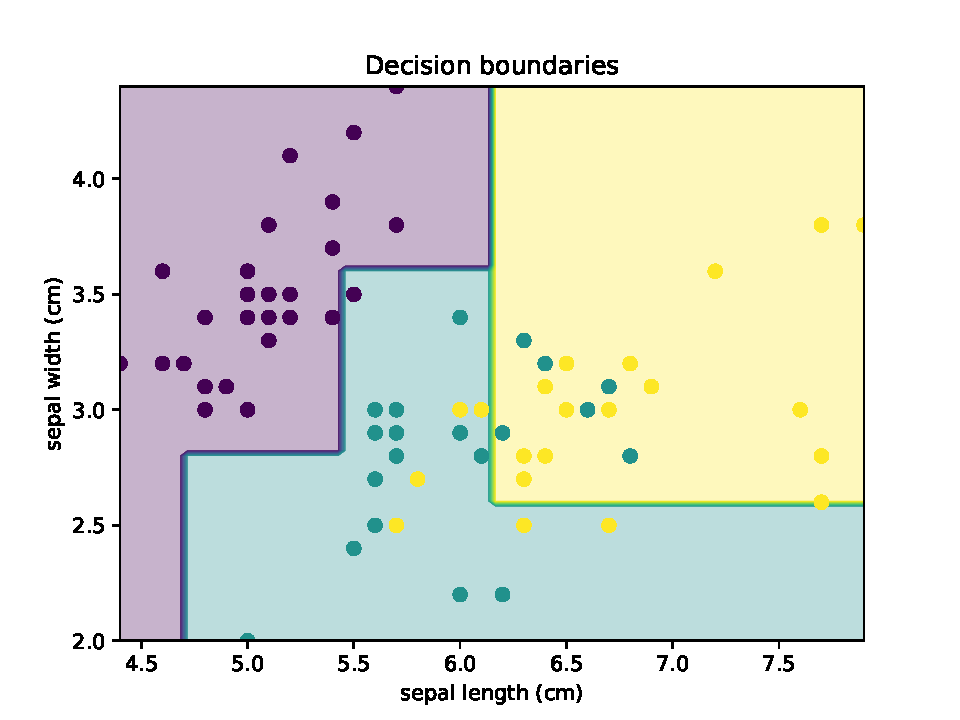
\includegraphics[width=\textwidth]{../plots/DB3.pdf}
            \caption{Περιοχές απόφασης του ταξινομητή και σημεία διασποράς που απεικονίζουν τα δείγματα χρωματισμένα σύμφωνα με την κλάση που ανήκουν πραγματικά}
            \label{fig:DB3}
    \end{figure}


\end{columns}
\end{frame}

\subsection{2η Ενότητα}
\begin{frame}{Ίριδα (Δέντρο Απόφασης/ Τυχαίο Δάσος)}
    Στη 2η Ενότητα χρησιμοποιούμε ταξινομητή \selectlanguage{english} RandomForest.\selectlanguage{greek}Συγκεκριμένα, εφαρμόζουμε τεχνική \selectlanguage{english} Bootstrap  \selectlanguage{greek} στο σύνολο εκπαίδευσης Α που χρησιμοποιήσαμε και στην προηγούμενη ενότητα (που είναι το μισό του αρχικού με τα 150 δείγματα) με αποτέλεσμα να καταλήγουμε με 100 νέα σύνολα που είναι σε μέγεθος μισά του Α. Για την αξιολόγηση του αλγορίθμου χρησιμοποιούμε πάλι το ίδιο με την 1η ενότητα. Τα 100 δέντρα που προκύπτουν έχουν όλα το ίδιο μέγιστο βάθος.
\end{frame}

\subsubsection{Ερώτημα 1}
\begin{frame}{Ίριδα (Δέντρο Απόφασης/ Τυχαίο Δάσος)}
    Χωρίς βελτιστοποίηση υπερπαραμέτρων, λαμβάνουμε ποσοστό σωστής ταξινόμησης 0.76, τιμή που δεν είναι ιδιαίτερα ικανοποιητική. Βελτιστοποιώντας, ωστόσο, ως προς το μέγιστο βάθος (κάθε δένδρου στο τυχαίο δάσος), πετυχαίνουμε ακρίβεια ίση με 0.8 για βάθος 3. Παρατηρούμε, συνεπώς, ότι το Τυχαίο Δάσος μας έδωσε καλύτερα αποτελέσματα από το Δένδρο Απόφασης, για το ίδιο φυσικά σύνολο δεδομένων.
\end{frame}

\subsubsection{Ερώτημα 2}
\begin{frame}{Ίριδα (Δέντρο Απόφασης/ Τυχαίο Δάσος)}
    \begin{columns}

    \column{0.48\textwidth}
        Από το διπλανό γράφημα συμπεραίνουμε ότι στην περίπτωση του Τυχαίου Δάσους, τα όρια απόφασης προσαρμόζουν καλύτερα στα δεδομένα και οι γραμμές είναι πιο \selectlanguage{english} "refined", \selectlanguage{greek} γεγονός που εξηγεί και το υψηλότερο ποσοστό σωστής ταξινόμησης που λάβαμε συγκριτικά με αυτό του Δένδρου Απόφασης. Ωστόσο, ενδεχομένως να υπάρχει και μεγαλύτερος κίνδυνος για \selectlanguage{english}overfitting.



    \column{0.48\textwidth}

    \begin{figure}
        \centering
            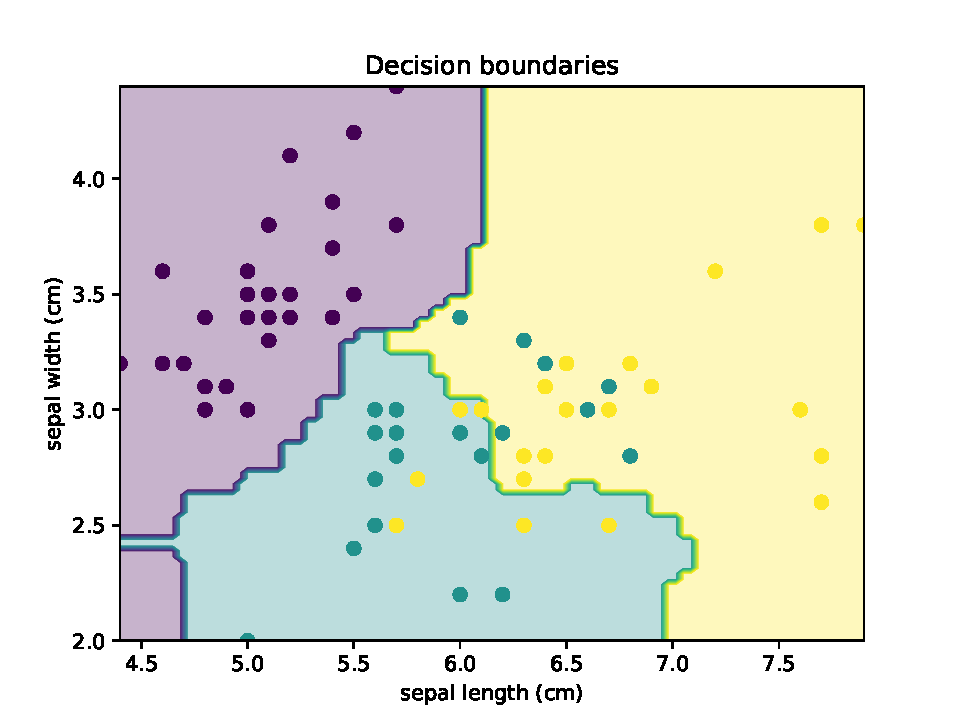
\includegraphics[width=\textwidth]{../plots/DB4.pdf}
            \caption{Περιοχές απόφασης του ταξινομητή και σημεία διασποράς που απεικονίζουν τα δείγματα χρωματισμένα σύμφωνα με την κλάση που ανήκουν πραγματικά}
            \label{fig:DB4}
    \end{figure}


\end{columns}
\end{frame}

\subsubsection{Ερώτημα 3}
\begin{frame}{Ίριδα (Δέντρο Απόφασης/ Τυχαίο Δάσος)}
    \begin{columns}

    \column{0.52\textwidth}
       Στο τελευταίο ερώτημα της ενότητας, εξετάζουμε πως μεταβάλλεται η απόδοση του αλγορίθμου συναρτήσει του \(\gamma\), όπου \(\gamma\) είναι το ποσοστό του συνόλου Α που χρησιμοποιείται κάθε φορά για κάθε δέντρο. Τρέξαμε τον αλγόριθμο για 100 τιμές $\gamma \in (0,1)$. Παραθέτουμε ένα γράφημα της μεταβολής του ποσοστού της ακρίβειας ταξινόμησης συναρτήσει του \(\gamma\). Παρατηρούμε ότι για πολύ μικρά $\gamma$ ($<0.1$) η ακρίβεια μειώνεται σημαντικά. Όμως για τις υπόλοιπες τιμές, η ακρίβεια αυξομειώνεται χωρίς αναγνωρίσιμο μοτίβο.



    \column{0.48\textwidth}

    \begin{figure}
        \centering
            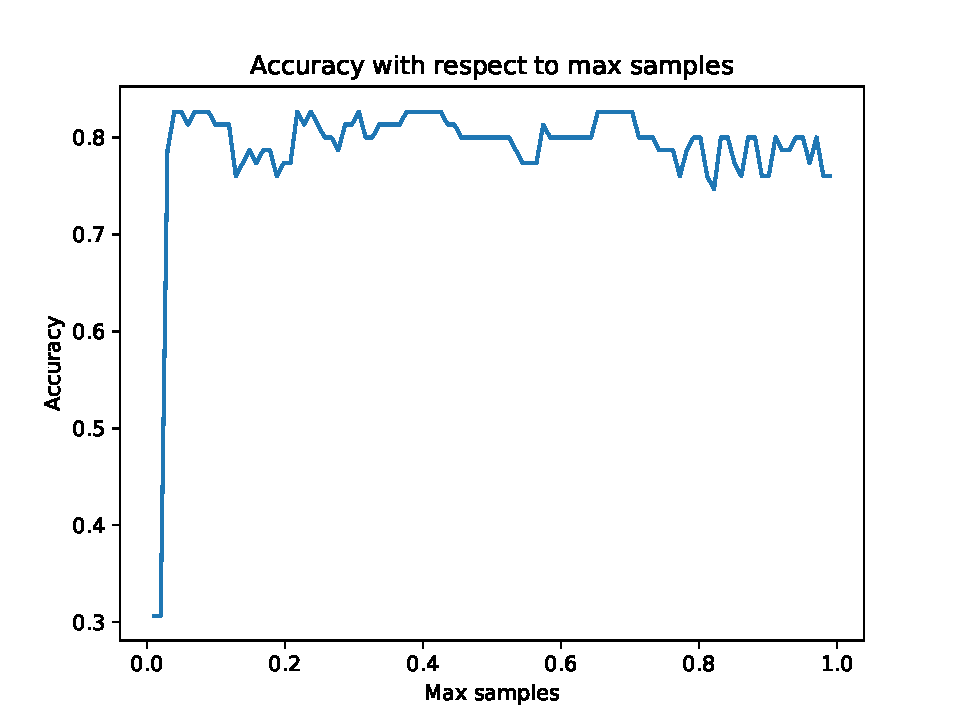
\includegraphics[width=\textwidth]{../plots/accuracy.pdf}
            \caption{Γράφημα ακρίβειας συναρτήσει της τιμής του \(\gamma\)}
            \label{fig:accuracy}
    \end{figure}


\end{columns}
\end{frame}




\section{ΜΕΡΟΣ Δ}
\subsection{Εισαγωγή}
\begin{frame}
    \frametitle{ΜΕΡΟΣ Δ - Εισαγωγή}
    \small
    Σε αυτό το κομμάτι της εργασίας μας δίνεται ένα \en training dataset \gr με 8743 δείγματα, 224 \en features \gr ανά δείγμα και οι ετικέτες για κάθε δείγμα/διάνυσμα χαρακτηρηστικών $(feature vector)$, συνολικά, ένας πίνακας διαστάσεων 8743 επί 225 με την τελευταία στήλη να είναι οι ετικέτες. Οι τιμές των ετικετών κυμαίνονται από 1,..,5, δηλαδή οι κλάσεις στις οποίες ταξινομούνται τα δείγματα είναι συνολικά 5. Προσπαθούμε να αναπτύξουμε έναν αλγόριθμο ταξινόμησης με όποια μέθοδο κρίνουμε ότι αποδίδει τα καλύτερα αποτελέσματα στον εν λόγω \en dataset. \gr Προκειμένου, να καταλήξουμε στο βέλτιστο μοντέλο, δοκιμάζουμε διάφορες διαδεδομένες τεχνικές εκπαίδευσης και ταξινόμησης, όπου προφανώς κάποιες εφαρμόζουν πολύ καλύτερα από κάποιες άλλες, δεδομένων των αριθμών των δειγμάτων μας και των αριθμών των διαστάσεων των \en feature \gr μας.
Αφού έχουμε εκπαιδεύσει και επαληθεύσει το μοντέλο μας, στη συνέχεια το εφαρμόζουμε σε ένα νέο \en test dataset \gr που αποτελείται από 6955 δείγματα και για τα οποία δεν γνωρίζουμε εκ των προτέρων την ετικέτα τους. Τέλος, εξάγουμε το διάνυσμα με τις ετικέτες που προέβλεψε το εκπαιδευμένο μοντέλο μας πάνω στα δείγματα του  \en test dataset. \gr
    
    
\end{frame}

\begin{frame}{Εισαγωγή}
    \gr
    Η υλοποίηση έγινε με έτοιμες συναρτήσεις της βιβλιοθήκης \en sklearn. \gr
    
    Για κάθε μοντέλο που δοκιμάστηκε, η επιλογή των υπερπαραμέτρων έγινε με τη χρήση της \en GridSearchCV. \gr
    Τα μοντέλα εκπαιδεύονται στο 80\% των δεδομένων με \en 3-fold cross validation, \gr και υπολογίζεται η απόδοση τους 
    στο υπόλοιπο 20\%. Γίνεται εκπαίδευση για κάθε υπερπαράμετρο στο \en param\_grid \gr που ορίζουμε εμέις, και επιστρέφεται το καλύτερο μοντέλο.
    
    Επειδή οι δοκιμές δεν έγιναν όλες ταυτόχρωνα (διότι αυτό θα επιθυμούσε πολύ χρόνο), αλλά δοκιμάζονταν διάφορες παράμετροι
    σε διαφορετικές κλήσεις του κώδικα, ο τελικός κώδικας \en python \gr περιέχει μόνο τις τελικές υπερπαραμέτρους στις οποίες καταλήξαμε. 

\end{frame} 



\begin{frame}{Εισαγωγή}
    Τα μοντέλα τα οποία δοκιμάστηκαν είναι τα εξίς: \en
\begin{itemize}
    \item Random Forest Classifier
    \item Gaussian Naive Bayes Classifier
    \item K-NN Classifier
    \item Suport Vector Classifier
    \item MLP Classifier
\end{itemize}
\gr
\end{frame}

\subsection{\en Random Forest Classifier}

\begin{frame}{\en Random Forest Classifier}
\gr
\begin{itemize}
        \item \textbf{Εκπαίδευση:} Κάθε δέντρο εκπαιδεύεται σε ένα διαφορετικό υποσύνολο των δεδομένων εκπαίδευσης, που δημιουργείται με τη μέθοδο \en bootstrapping\gr. Για κάθε κόμβο, η επιλογή του καλύτερου χαρακτηριστικού γίνεται με τυχαία υποσύνολα χαρακτηριστικών.
        \item \textbf{Πρόβλεψη:} Για ένα νέο δείγμα, κάθε δέντρο κάνει μια πρόβλεψη. Ο \en Random Forest \gr συνδυάζει τις προβλέψεις αυτές μέσω ψηφοφορίας για την ταξινόμηση, όπου και μας ενδιαφέρει.
        \item \textbf{Αντιμετώπιση υπεράρμωσης:} Η τυχαιότητα που εισάγεται τόσο στα δεδομένα όσο και στα χαρακτηριστικά μειώνει την πιθανότητα υπεράρμωσης (\en overfitting).  \gr
        \item \textbf{Πλεονεκτήματα:} Ο \en Random Forest \gr είναι ιδιαίτερα αποτελεσματικός σε προβλήματα με πολλές μεταβλητές, αλληλεπιδράσεις ή δεδομένα με ελλείψεις.
    \end{itemize}

    Ο \en Random Forest \gr είναι ένα μοντέλο που προσφέρει καλή απόδοση χωρίς να απαιτεί σημαντική παραμετροποίηση και είναι κατάλληλο για πολλές εφαρμογές.
\end{frame}


\begin{frame}{\en Random Forest Classifier \gr Αποτελέσματα}
\gr
    \begin{itemize}
        \item Συνάρτηση: $ RandomForestClassifier()$
        \item Υπερπαράμετροι που δοκιμάστηκαν: \begin{enumerate}
            \item $n\textunderscore estimators=\{100,200,300,400,500\} (default = 100)$
            \item $criterion = \{gini, entropy, log\textunderscore loss \}(default = gini)$
            \item $max\textunderscore depth =\{ 5, 10, 20, 30, None\} (default=None)$
            \item $max\textunderscore features = \{sqrt, log2, None\} (default = sqrt)$
        \end{enumerate}
        \item \en Accuracy: 0.8147512864493996
        \item \gr Τελικές υπερπαράμετροι: \en
        \begin{itemize}
            \item $n\_estimators = 300$
            \item defaults
        \end{itemize}
    \end{itemize} \gr
\end{frame}



\subsection{\en Gaussian Naive Bayes Classifier}

\begin{frame}{\en Gaussian Naive Bayes Classifier}
\gr
Χρησιμοποιήθηκε η συνάρτηση $GaussianNB()$. 

Πρόκειται για έτοιμη υλοποίηση του μοντέλου Μπεϋζιανής ταξινόμησης. Συγκεκριμένα, επειδή στη μέθοδο αυτή πρέπει να 
γνωρίζουμε εκ των προτέρων την συνάρτηση πυκνότητας πιθανότητας, η ρουτίνα αυτή υποθέτει γκαουσιανή κατανομή. 

Περιμένουμε να μην έχει πολύ καλά αποτελέσματα διότι δεν έχουμε κανένα λόγο να πιστεύουμε ότι τα συγκεκριμένα δεδομένα
ακολουθούν γκαουσιανή κατανομή. Όμως, εφόσον δεν γνωρίζουμε τίποτα για τη φύση των δεδομένων (τι υποδηλώνουν, από που δειγματοληπτήθηκαν, τη πυκνότητα πιθανότητας τους) δεν μπορούμε να κάνουμε κάποια καλύτερη υπόθεση. 
    
\end{frame}

\begin{frame}{\en Gaussian Naive Bayes Classifier \gr Αποτελέσματα}
\gr
    \begin{itemize}
        \item Συνάρτηση:  $GaussianNB()$
        \item Υπερπαράμετροι που δοκιμάστηκαν: Καμία
        \item \en Accuracy: 0.6986849628359062
    \end{itemize} \gr
    
\end{frame}


\subsection{\en K-NN Classifier}


\begin{frame}{\en K-NN Classifier}
\gr
Ο \en K-Nearest Neighbors (K-NN)\gr είναι ένας απλός αλλά αποτελεσματικός ταξινομητής που βασίζεται στη γειτνίαση των δεδομένων. Η βασική ιδέα του K-NN είναι ότι παρόμοια δείγματα τείνουν να ανήκουν στην ίδια κλάση.

    \begin{itemize}
        \item \textbf{Εκπαίδευση:} Ο K-NN δεν απαιτεί εκπαίδευση με την παραδοσιακή έννοια. Αντίθετα, αποθηκεύει ολόκληρο το σύνολο δεδομένων εκπαίδευσης και το χρησιμοποιεί για πρόβλεψη.
        \item \textbf{Πρόβλεψη:} Για ένα νέο δείγμα:
        \begin{enumerate}
            \item Υπολογίζει την απόσταση του νέου δείγματος από κάθε σημείο του συνόλου εκπαίδευσης (συνήθως χρησιμοποιείται η Ευκλείδεια απόσταση).
            \item Επιλέγει τους $k$ πιο κοντινούς γείτονες.
            \item Η κλάση της πρόβλεψης καθορίζεται από την πλειοψηφία των γειτόνων για  την ταξινόμηση.
        \end{enumerate}
    \end{itemize}
\end{frame}

\begin{frame}{\en K-NN Classifier}
\begin{itemize}
    \item \textbf{Πλεονεκτήματα:} Δεν απαιτεί εκπαίδευση, και είναι κατάλληλος για δεδομένα με μη γραμμικούς διαχωρισμούς.
        \item \textbf{Μειονεκτήματα:} Η πρόβλεψη μπορεί να είναι αργή για μεγάλα σύνολα δεδομένων, ενώ είναι ευαίσθητος στην κλιμάκωση των χαρακτηριστικών.
\end{itemize}
    Ο K-NN είναι ιδανικός για μικρά και μεσαία σύνολα δεδομένων, ειδικά όταν οι σχέσεις μεταξύ των δειγμάτων είναι σαφείς και μπορούν να αναπαρασταθούν γεωμετρικά.

\end{frame}

\begin{frame}{\en K-NN Classifier \gr Αποτελέσματα}
\gr
        \begin{itemize}
        \item Συνάρτηση: $KNeighborsClassifier()$
        \item Υπερπαράμετροι που δοκιμάστηκαν: \begin{enumerate}
            \item $n\_ neighbors=\{5,10,14,16\}(default = 5)$
            \item $weights=\{uniform,distance\}(default = uniform)$
            \item $algorithm = \{auto, ball\_ tree, kd\_ tree, brute\}(default = auto)$
            \item $p=\{1,2\}(default = 2)$
        \end{enumerate}
        \item \en Accuracy:  0.8416237850200115
        \item \gr Τελικές υπερπαράμετροι: \en
        \begin{itemize}
            \item $n\_neighbors = 14$
            \item $p = 1$
            \item $weights=distance$
            \item defaults
        \end{itemize}
    \end{itemize} \gr
\end{frame}



\subsection{\en Suport Vector Classifier}


\begin{frame}{\en Suport Vector Classifier}
\scriptsize
\gr
Ο \en Support Vector Classifier (SVC) \gr είναι μια μέθοδος μηχανικής μάθησης που ανήκει στην οικογένεια των \en Support Vector Machines (SVMs)\gr και χρησιμοποιείται για προβλήματα ταξινόμησης. Η βασική ιδέα του \en SVC \gr είναι να βρει έναν υπερεπίπεδο που διαχωρίζει τις κλάσεις με τον καλύτερο δυνατό τρόπο.

    \begin{itemize}
        \item \textbf{Βασική Αρχή:}
        \begin{itemize}
            \item Ο \en SVC \gr αναζητά το υπερεπίπεδο που μεγιστοποιεί το περιθώριο \en (margin), \gr δηλαδή την ελάχιστη απόσταση μεταξύ του υπερεπιπέδου και των πιο κοντινών σημείων κάθε κλάσης (\en support vectors). \gr
            \item Στόχος είναι η εύρεση ενός γραμμικού ή μη γραμμικού διαχωρισμού ανάμεσα στις κλάσεις.
        \end{itemize}

        \item \textbf{Επεκτάσεις για μη γραμμικά προβλήματα:}
        \begin{itemize}
            \item Χρησιμοποιείται η τεχνική του \en \textit{kernel trick}\gr, που επιτρέπει τη μετατροπή των δεδομένων σε υψηλότερες διαστάσεις για να γίνουν γραμμικά διαχωρίσιμα.
            \item Συχνά χρησιμοποιούμενοι πυρήνες \en (\textit{kernels}):  \gr
            \begin{itemize}
                \item Γραμμικός (\en \textit{linear kernel})\gr
                \item Πολυωνυμικός (\en \textit{polynomial kernel})\gr
                \item \en Radial Basis Function (RBF)
            \end{itemize}
        \end{itemize}
        \end{itemize}
\end{frame}

\begin{frame}{\en Support Vector Classifier}
\begin{itemize}
        \item \textbf{Πλεονεκτήματα:}
        \begin{itemize}
            \item Κατάλληλος για μικρά και μεσαία σύνολα δεδομένων.
            \item Αποτελεσματικός ακόμα και με υψηλής διάστασης δεδομένα.
        \end{itemize}

        \item \textbf{Μειονεκτήματα:}
        \begin{itemize}
            \item Μπορεί να είναι αργός για πολύ μεγάλα σύνολα δεδομένων.
            \item Η επιλογή κατάλληλων παραμέτρων ($C$, $γ$) και πυρήνα είναι κρίσιμη.
        \end{itemize}
\end{itemize}

    Ο \en SVC \gr είναι ιδανικός για προβλήματα ταξινόμησης όπου απαιτείται υψηλή ακρίβεια και οι κλάσεις δεν είναι εύκολα διαχωρίσιμες γραμμικά.
\end{frame}



\begin{frame}{\en Suport Vector Classifier \gr Αποτελέσματα}
\gr
        \begin{itemize}
        \item Συνάρτηση: $SVC()$
        \item Υπερπαράμετροι που δοκιμάστηκαν: \begin{enumerate}
            \item $C=\{10,100,1000\}$
            \item $\gamma=\{0.1,0.01,0.001\}$
            \item $kernel = \{linear, poly, rbf, sigmoid\}$
            \item $class\_weight = \{dict, balanced, None\}$
        \end{enumerate}
        \item \en Accuracy:  0.8650657518582047
        \item \gr Τελικές υπερπαράμετροι: \en
        \begin{itemize}
            \item $C=10$
            \item $class\_weight = balanced$
            \item $\gamma=0.01$
            \item $kernel=poly$
            \item defaults
        \end{itemize}
    \end{itemize} \gr
\end{frame}





\subsection{\en MLP Classifier}

\begin{frame}{\en Multi-Layer-Perceptron Classifier}
\gr
Χρησιμοποιήθηκε η συνάρτηση $MLPClassifier()$.

Πρόκειται για έτοιμη υλοποίηση ενός νευρωνικού δικτύου που εκπαιδεύεται με τη μέθοδο του \en backpropagation. \gr

Είναι ίσως το πιο γενικό μοντέλο που δοκιμάστηκε, μιας και μπορει με κατάλληλες υπερπαραμέτρους να προσεγγίσει οποιαδήποτε συνάρτηση. Επομένως περιμένουμε πολύ καλά αποτελέσματα. 

\begin{itemize}
    \item \textbf{Βασική Δομή:}
        \begin{itemize}
            \item Αποτελείται από τρία βασικά επίπεδα:
            \begin{itemize}
                \item \textbf{Είσοδος (\en Input Layer \gr):} Παίρνει τις εισόδους (χαρακτηριστικά των δεδομένων).
                \item \textbf{Κρυφά Επίπεδα (\en Hidden Layers \gr):} Περιέχουν νευρώνες που μαθαίνουν μη γραμμικές σχέσεις.
                \item \textbf{Έξοδος (\en Output Layer \gr):} Παράγει τις τελικές προβλέψεις (π.χ. πιθανότητες για κάθε κλάση).
            \end{itemize}
            \item Οι νευρώνες κάθε επιπέδου είναι πλήρως συνδεδεμένοι με τους νευρώνες του επόμενου επιπέδου.
        \end{itemize}
\end{itemize}

\end{frame}


\begin{frame}{\en Multi-Layer-Perceptron Classifier}

     \begin{itemize}


        \item \textbf{Μηχανισμός Μάθησης:}
        \begin{itemize}
            \scriptsize
            \item Χρησιμοποιείται η μέθοδος της \textbf{προώθησης \en (forward propagation)} \gr για τον υπολογισμό της εξόδου.
            \item Ο υπολογισμός των σφαλμάτων γίνεται με τη χρήση της συνάρτησης κόστους (π.χ. \en cross-entropy loss \gr για ταξινόμηση).
            \item Η \textbf{οπισθοδιάδοση \en (backpropagation)} \gr ενημερώνει τα βάρη με βάση το σφάλμα μέσω του αλγορίθμου \en gradient descent. \gr
        \end{itemize}


        \item \textbf{Πλεονεκτήματα:}
        \begin{itemize}
            \scriptsize
            \item Μπορεί να μάθει πολύπλοκα μοτίβα στα δεδομένα.
            \item Προσαρμόζεται καλά σε μεγάλα σύνολα δεδομένων.
        \end{itemize}

        \item \textbf{Μειονεκτήματα:}
        \begin{itemize}
            \scriptsize
            \item Απαιτεί σημαντικούς υπολογιστικούς πόρους.
            \item Υπάρχει κίνδυνος υπεράρμωσης \en (overfitting) \gr αν δεν γίνει καλή ρύθμιση.
        \end{itemize}
    \end{itemize}

    Ο \en MLP \gr είναι ένα ευέλικτο εργαλείο για προβλήματα ταξινόμησης, αλλά απαιτεί σωστή παραμετροποίηση για βέλτιστα αποτελέσματα.
\end{frame}

\begin{frame}{\en Multi-Layer-Perceptron Classifier \gr Αποτελέσματα}
\gr
    \begin{itemize}
        \item Συνάρτηση: $MLPClassifier()$
        \item Υπερπαράμετροι που δοκιμάστηκαν: \en
        \begin{itemize}
            \item $hidden\_layer\_sizes = \{(10),(20),(30),(40),(50),(60),(70),(80),(90),(100),(500),(10000), $ $
            (30,30),(40,40),(50,50),(100,100), $ $
            (100,10),(200,20),(400,36),(500,50), $ $
            (10,100,10),(20,100,20),(50,500,50)\}, default = (100)$
            \item $activation = \{ 'logistic', 'tanh', 'relu' \}, default='relu'$
            \item $solver = \{'lbfgs', 'sgd', 'adam'\}, (default = 'adam')$
            \item alpha = linear space between (0.000001, 100), $default = 0.0001$
            \item $learning\_rate = \{'comstant', 'adaptive' \}, default = 'constant'$
        \end{itemize}
        \item \en Accuracy: 0.8502001143510578 
        \item \gr Τελικές υπερπαράμετροι: \en
        \begin{itemize}
            \item $hidden\_layer\_sizes=(400,36)$
            \item defaults
        \end{itemize}
        \gr

        Ίσως με κατάλληλες υπερπαραμέτρους να μπορεί να βελτιωθεί περαιτέρω.
    \end{itemize} \gr

\end{frame}




\subsection{Σύγκριση Μοντέλων}
\begin{frame}{Σύγκριση Μοντέλων}
\en
\small
\begin{table}[]
\centering
\begin{tabular}{|l|c|}
\hline
\textbf{\gr Μοντέλο}                      & \textbf{\en Accuracy } \\ \hline
\textbf{Random Forest Classifier}    & 0.8147512864493996 \\ \hline
\textbf{Gaussian Naive Bayes}        & 0.6986849628359062 \\ \hline
\textbf{K-NN Classifier}             & 0.8416237850200115 \\ \hline
\textbf{Support Vector Classifier}   & 0.8650657518582047 \\ \hline
\textbf{MLP Classifier}              & 0.8502001143510578 \\ \hline
\end{tabular}
\label{tab:model_accuracy}
\end{table} \gr


Όπως φαίνεται στον πίνακα, τα καλύτερα αποτελέσματα πάρθηκαν μέσω του μοντέλου \en support vector classifier. \gr
Κάθε ένα από τα μοντέλα ενδέχεται να είχε καλύτερα αποτελέσματα με κατάλληλη επιλογή υπερπαραμέτρων. Ειδικότερα το νευρωνικό δίκτυο θα έπρεπε να έχει εξίσου καλά αποτελέσματα με το \en support vector \gr όμως δεν βρέθηκαν οι κατάλληλες υπερπαράμετροι.

Η διαφορά στο \en accuracy \gr μπορεί επίσης να οφείλεται σε ιδιαιτερότητες του \en test set, \gr 
και δεν είναι απαραίτητο ότι το \en support vector \gr θα έχει τα καλύτερα αποτελέσματα στο \en dataset \gr 
που μας δόθηκε να κάνουμε την πρόβλεψη. 



\end{frame}


\begin{frame}{Κατάληξη}

Η ταξινόμηση των τελικών αποτελεσμάτων έγινε με το \en support vector \gr μοντέλο, με υπερπαραμέτρους:
\en
\begin{itemize}
    \item C = 10
    \item gamma = 0.01
    \item kernel = 'poly'
    \item class\_weight = 'balanced'
\end{itemize}
\gr

Ό,τι προσπάθεια και να κάναμε, δεν καταφέραμε να υπερβούμε το κατόφλι των $\sim 85\%$. Ύποθέτουμε, έτσι, ότι υπήρχε κάποια επικάλυψη των κλάσεων, ώστε ήταν να είναι αδύνατη η ακριβέστερη ταξινόμηση χωρίς επιπλέον \en features. \gr

Ελπίζουμε να μην έπεσε θύμα της υπεράρμωσης, αφού χρησιμοποιήσαμε \en 3-fold cross valitation \gr στην εκπαίδευση του και η αξιολόγησή του έγινε σε ξεχωριστό σετ δεδομένων. 

Τα αποτελέσματα αποθηκεύτηκαν στο αρχείο \en labels30.npy. \gr 
Μπορείτε να βρείτε την δουλειά μας στο \en github \gr \href{https://github.com/bilonio/ProjectML.git}{εδώ}.

\end{frame}


\end{document}